\chapter {Graficzny interfejs użytkownika i instrukcja obsługi}
\label{cha:gui}
Poniższy rozdział zawiera opis Graficznego Interfejsu Użytkownika oraz wskazówki i przykłady jak z niego korzystać
w sposób efektywny.
Interfejs użytkownika, przedstawiony na rysunku \ref{gui_cale} 
\begin{figure}
\begin{center}
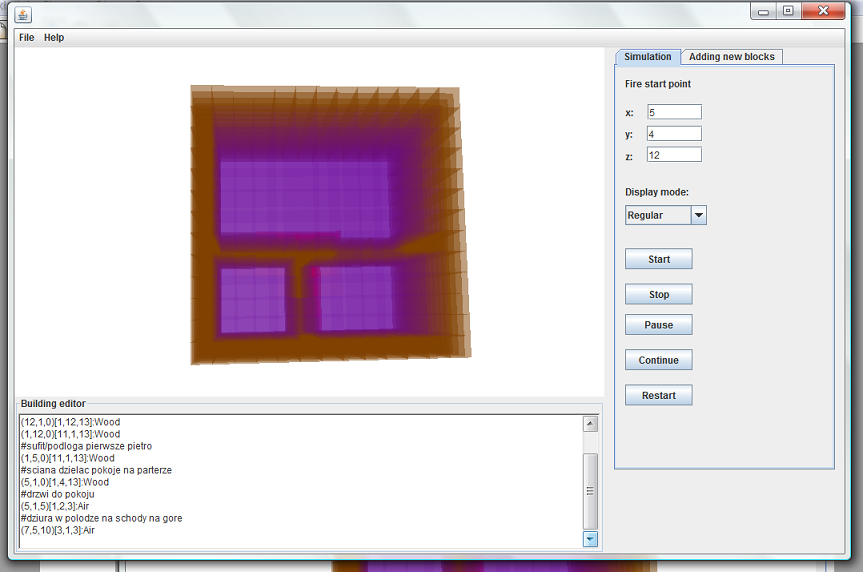
\includegraphics{gui_cale.png} 
\caption { Graficzny interfejs użytkownika}
\label {gui_cale}
\end{center}
\end{figure}
W celu zapewnienia wygody i efektywności pracy został podzielony na następujące części:
\begin {enumerate}
\item Panel górny
\item Widok scenmy
\item Menu boczne
\item Edytor
\end {enumerate}
\section{Panel górny}
Panel górny zawiera elementy:
\begin{itemize}
\item File, składający się z pozycji:
\begin{itemize}
\item Save cell states - zapis stanu komórek automatu do pliku. Automat zapisany jest w postaci zbioru macierzy dwuwymiarowych, z których każda przedstawia jeden poziom automatu począwszy od poziomu 0 zgodnie z osią Y.
\item Save temperatures - zapis rozkładu temperatur automatu. Format zapisu identyczny z przypadkiem stanu komórek.
\item Read building from file - możliwość wczytania budynku z pliku. Format zapisu budynku w pliku jest taki sam jak w edytorze.
	Po wczytaniu budynku z pliku, jego opis pojawia się w edytorze co pozwala na dalsze modyfikacje.
\end {itemize}
\item Help, skonstruowany z opcji:
\begin {itemize}
\item User guide - podstawowe informacje o użytkowaniu programu: jak korzystać z edytora oraz panelu bocznego.
\item About program - podstawowe informacje o programie.
\end {itemize}
\end{itemize}

\section{Scena}
Główny elementem interfejsu jest scena, przedstawiająca wyniki symulacji. Aplikacja dostarcza możliwość manipulowania sceną w celu zróżnicowania widoku. Możliwe są do wykonania następujące akcje:
\begin {itemize}
\item Oddalanie i przybliżanie sceny za pomocą strzałek klawiatury. Strzałka w górę powoduje przybliżenie, zaś strzałka w dół oddalenie.
\item Obrót elementów na scenie za pomocą strzałek w bok. Strzałka w prawo obraca scenę zgodnie z ruchem wskazówek zegara, zaś strzałka w lewo przeciwnie do ich ruchu.
\end {itemize}

\section{Edytor}
Elementem wykorzystywanym do edycji budynku jest umieszczony na dole interfejsu edytor.
Edytor, jak zostało to opisane w rozdziale \ref{cha:implementacja} jest polem tekstowym i jako takie umożliwia
 operacje zaznaczania, kopiowania, wklejania i usuwania tekstu za pomocą standardowych skrótów klawiaturowych.
 Tekts umieszczany w edytorze służy do konstrukcji budynku, w którym przeprowadzana jest symulacja pożaru i powinien być zgodny z następującym formatem:
 \begin{enumerate}
 \item Konieczne jest aby każdy element konstrukcyjny był zapisany w osobnej linii.
 \item Pojedynczy, dodawany element jest ortogonalnym, jednolitym blokiem o następującej postaci:
 \begin{center}
	(Start\_X,Start\_Y,Start\_Z)[Rozmiar\_X,Rozmiar\_Y,Rozmiar\_Z]:Material
 \end {center}
 gdzie:
	 \begin{itemize}
	 \item (Start\_X,Start\_Y,Start\_Z) - są to adekwatnie współrzędne (X,Y,Z) Lewego-Dolnego-Tylnego wierzchołka bloku, będącego początkiem bloku co przedstawia rysunek \ref{osie}. 
	 \item $[$Rozmiar\_X,Rozmiar\_Y,Rozmiar\_Z$]$ - określają rozmiar wprowadzanego bloku. 
	 \item Komórki w automacie numerwane są od 0. Wszystkie współrzędne są całkowitymi liczbami nieujemnymi i oznaczają wielokrotność komórek w danej osi.
	 \item Materiał jest nazwą jednego z dostępnych materiałów. Dostępne materiały to:
	 \begin {itemize}
	 \item Drewno
	 \item Metal
	 \item Cegła
	 \item Powietrze
	 \end {itemize}
	 Blok zbudowany z materiału powietrze, może być wykorzystany do wstawienia dziury w ścianie lub podłodze odpowiadającej oknu lub przejściu na wyższe piętro budynku.
	 \end{itemize}
\item Linia rozpoczynająca się od znaku # jest traktowana jako komentarz i nie podlega analizie.
 \end {enumerate}
 \begin{figure}
\begin{center}
\includegraphics{osie.jpg} 
\caption { Orientacja bloku}
\label {osie}
\end{center}
\end{figure}
\section{Panel boczny}
Panel boczny składa się z dwóch zakładek:
\begin {enumerate}
\item Zakładka \textit{Simulation} dostarcza opcje pozwalające kontrolować przebieg symulacji.
\begin {itemize}
	\item Trzy pola tekstowe oznaczone etykietami \textit{x},\itextit{y} i \textit{z} pozwalają podać współrzędne bloku, w którym rozpoczyna się pożar.
	\item Pole wyboru trybu \textit{Diplay mode} przełącza scenę w jeden z dwóćh trybów:
	\begin{itemize}
	\item Tryb regularny - domyślny tryb, w którym pokazany jest aktualny stan komórki. Komórka będą w stanie naturalnym zachowuje kolor i przeźroczystość materiału z którego została stworzona. Komórka paląca się ma kolor czerwony. Dym przedstawiony jest jako szary.
	\item Tryb temperaturowy - przedstawia rozkład temperatur w budynku. Kolor niebiskie oznacza temperaturę z zakresu $[20-50^\circ C]$. Temperatury powyżej $50^\circ C$ przedstawione są w odcieniach czerwieni. Im intensywniejsza czerwień, tym większa temperatura.
\end{itemize}
	\item Guziki \textit {Start}, \textit{Stop}, \textit{Pause}, \textit{Continue}, \textit {Restart} pozwalają na kontrolowanie symulacji. Umożliwiają na przykład zatrzymanie pracy automatu w celu zapisu wyników pośrednich lub modyfikacji budynku, a następnie wznowienie działania.
	\end{itemize}
\item Zakładka \textit{Adding new blocks} jest alternatywą \textit{Edytora}. Umożliwia edycję budynku i jest przydatna szczególnie dla osób nieobytych z tekstowymi narzędziami pracy. Omawiana zakładka składa się z:
\begin {itemize}
\item Pola umowżliwiającego wybór materiału dla dodawanego bloku.
\item Pól tekstowych pozwalających wpisać współrzędne punktu startu dodawanego bloku oraz jego rozmiar.
\item Przycisku \textit{Add}, którego kliknięcie powoduje zaakceptowanie wprowadzonych zmian i utworzenie bloku.
\end {itemize}
\end {enumerate}
 

